\section{Compressione JPEG}
JPEG (Joing Photographic Experts Group) è lo standard di memorizzazione delle immagini fotografiche, che permette un'elevata compressione lossy con accettabile degradazione della qualità. 

JPEG definisce una serie di elaborazioni flessibili da seguire sulle immagini, che possono eventualmente essere saltate. Le regole sono però definite in modo rigido, includendo la decompressione.

\begin{figure}[h]
	\centering
	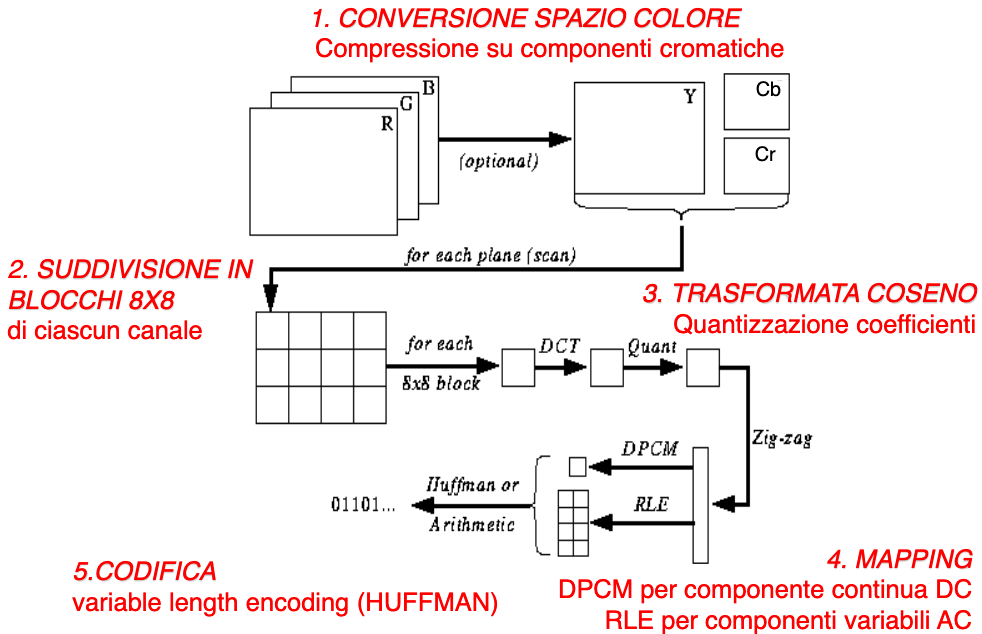
\includegraphics[scale=0.44]{Lezioni/Immagini/jpeg}
\end{figure}

La compressione JPEG si articola in 5 fasi:
\begin{enumerate}
	\item Conversione spazio colore, comprimendo le parti cromatiche;
	\item Suddivisione in blocchi 8$\times$8;
	\item Trasformata coseno e quantizzazione coefficienti;
	\item Mapping con DCPM e RLE;
	\item Codifica con Huffman.
\end{enumerate}
La perdita avviene nelle fasi di sottocampionamento del chroma e quantizzazione. 

\subsection{Conversione spazio cromatico}
Si può sfruttare la caratteristica psicovisuale per cui il sistema visivo umano è più sensibile alle variazioni di luminanza che non a quelle di crominanza, quantizzando maggiormente queste ultime.

In questo modo, la ridondanza psicovisuale diminuisce, con poca perdita. L'immagine viene convertita da RGB a un altro spazio come YCbCR, esprimendo il colore in termini di $x : y : z$ e campionando orizzontalmente.

La compressione lossy sulle coordinate cromatiche è opzionalmente effettuata riducendo le dimensioni sottocampionando tramite media a due a due tra i pixel adiacenti. 

\subsection{Suddivisione in blocchi}
Ciascun canale (Y, Cb, Cr) dell'immagine è diviso in blocchi quadrati, di cui ciascuno è costituito da 8$\times$8 pixel. 

\subsection{Analisi in frequenza}
L'idea per la quantizzazione si basa sull'utilizzo di una matrice dei coefficienti che genera coefficienti quantizzati. Le frequenze vengono pesate diversamente tagliando le alte frequenze, quindi dividendo con valori più alti, e salvando le basse applicando valori bassi.

In JPEG viene utilizzata la DCT, e i coefficienti rappresentano le ampiezze dei segnali armonici che sommati ricostruiscono il segnale.
$$F(u, v) = \sum_{x=0}^{M-1}\sum_{y=0}^{N-1} f(x, y) g(u, v, x, y)$$
$$f(x, y) = \sum_{u=0}^{M-1}\sum_{x=0}^{N-1} F(u, v) \cos\bigg[\frac{(2x + 1)\pi u}{2N}\bigg] \cos\bigg[\frac{(2x + 1)\pi v}{2N}\bigg]$$
$$g(x, y, u, v) = \alpha(u) \alpha(v) \cos\bigg[\frac{(2x + 1)\pi u}{2N}\bigg] \cos\bigg[\frac{(2y + 1)\pi v}{2N}\bigg]$$

Per ogni canale, a ogni blocco nello spazio corrisponde un blocco di coefficienti nel dominio della frequenza, in cui le basse frequenze sono in alto a sinistra e le alte sono in basso a destra. Il primo coefficiente del blocco trasformato è correlato al valore medio dei valori del blocco originario.

Viene poi definita una tabella di quantizzazione $Q$ che divide la matrice dei coefficienti $F$ e genera coefficienti quantizzati:
$$\hat{F}(u, v) = \text{round} \bigg(\frac{F(u, v)}{Q(u, v)}\bigg)$$
Le tabelle $Q(u, v)$ sono calcolate tramite esperimenti psicovisuali, scegliendo numeri che permettono una minore complessità computazionale. 

Poiché i valori della tabella di quantizzazione sono abbastanza elevati, i coefficienti quantizzati sono più piccoli e con una varianza minore. Si può variare il rapporto di compressione riscalando la tabella di quantizzazione (quality factor), che vengono poi moltiplicati in fase di decodifica:
$$ \tilde{F}(u, v) = \hat{F}(u, v) Q(u, v)$$
I coefficienti quantizzati sono ottenuti arrotondando all'intero più vicino, e quelli meno significativi tendono ad azzerarsi. 

Nelle regioni disomogenee (texture), i valori adiacenti sono distinti fra loro, e i coefficienti della matrice saranno in quantità maggiore e molto distanti dallo zero. A parità di coefficienti, la perdita è più elevata. La qualità, in generale, è buona con 16 coefficienti diversi da zero.

\subsection{Mapping dei coefficienti}
Il tipo di mapping impiegato si differenzia per i coefficienti supersititi, che possiedono una componente continua, indicata come DC, e alcune variabili, AC. Queste ultime vengono ordinate tramite zig-zag scan e codificati con RLE.

Sul valore DC invece viene applicata una tecnica DCPM (Differential Pulse Code Modulation), che codifica ogni blocco come differenza rispetto al valore del blocco precedente, sfruttando la correlazione statistica.
$$\delta_k = DC(0, 0)_k - DC(0, 0)_{k-1}$$

\subsection{Codifica dei dati}
L'ultima codifica applicata ai dati utilizza VLE (lunghezza variabile) in base all'entropia. Viene analizzata la frequenza statistica di ciascuna parola e a ognuna è assegnata una stringa del codice. 
$$p_r(r_k) = \frac{n_k}{n} \qquad L_{avg} = \sum_{k=0}^{L-1} l(r_k)p_r(r_k)$$

\begin{itemize}
	\item Codifica sequenziale: i blocchi DCT sono codificati e tramessi uno dopo l'altro, alternando le diverse componenti a colori (pagine web);
	\item Codifica progressiva: vengono trasmesse prima le porzioni più significative, visualizzando un'anteprima con qualità ridotta.
\end{itemize}

Per misurare la qualità della compressione, si usa il rapporto di compressione $C = \frac{bit_1}{bit_2}$ oppure il numero di bit per pixel. Questi valori sono dipendenti dal fattore di qualità. 

\subsection{JPEG-20}
La compressione con bit-stream ha una bassa complessità ed è efficiente, ma non esistono regioni di interesse e non è possibile differenziare la qualità.

JPEG-20 permette diverse risoluzioni, evitando i blocking artifact sfruttando una decomposizione wavelet a 3 livelli. A parità di fattore di compressione, l'immagine appare con meno blocchetti, quindi migliore.

Le zone più importanti, o meno uniformi, possono essere prioritizzate in termini di qualità, applicando una maggior compressione sullo sfondo.



